\chapter{System Design}
\label{cha:sysdesign}

To advance in this project we have mainly been programming, designing and developing the application. The programming language of choice is Adobe ActionScript and the IDE Flash Builder, which is very similar to the IDE Eclipse. The interface developed have multiple functionalities but misses some of the initially wanted functionalities. One of those functionalities that was not implemented is making the interface accept incoming video streams tagged with a location and cardinal direction from expected sources. The video streams will have to be tagged with these geographical datas somehow, which is not a common included feature with most video recording softwares. Developing a separate recording application to create these kind of geo-tagged video streams, for the sake of this project, was outside the scope of the thesis. Instead, we have in this thesis proved the functionality of our interface with synthetically generated video geo-tags. These streams have been made to work with the custom OSMF player.  Under-the-hood features desired for our media player include HAS in order to ensure a smooth playback of the streams, both for buffering a single stream but also for prefetching and buffering a fraction of the other streams to ensure uninterrupted playback during stream swaps. To help us focus on the main problem of developing this interface, we have been provided with some existing code by our supervisors. This includes a working SMP player created with a modified version of OSMF with code from an existing HAS-interface using prefetching \cite{qualbranch}.

\section{Interface Design}
\label{sec:interfacedesign}

The main part of this project is to expand upon the existing user interface (UI) of the default SMP player, as seen in Figure \ref{fig:mediaplayer}, and create a new section of it where we can implement the new desired functionality for this project. 

\begin{figure}[ht!]
\begin{center}
	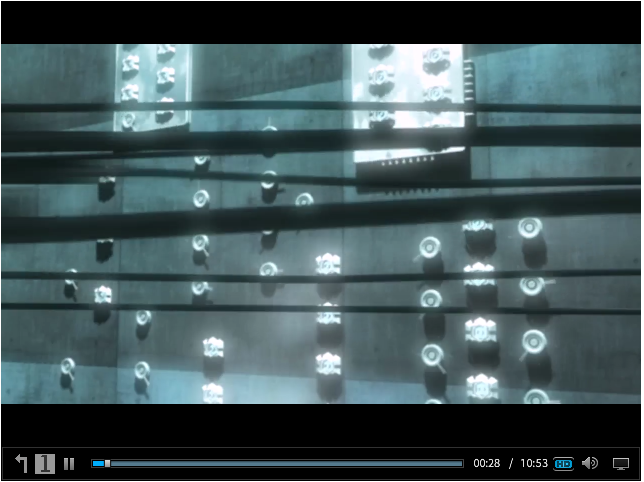
\includegraphics[scale=0.7]{Media_player.png}
	\caption{Strobe Media Player}
	\label{fig:mediaplayer}
\end{center}
\end{figure}

\begin{figure}[ht!]
\begin{center}
	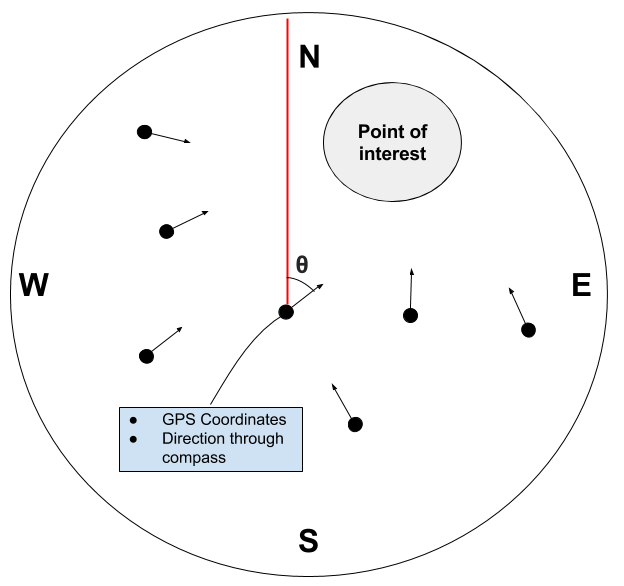
\includegraphics[scale=0.6]{teomet.png}
	\caption{Conceptual interface of GPS and Direction selection map}
	\label{fig:gpsinterface}
\end{center}
\end{figure}

For our interface design we decided to add an additional button to the control bar of the UI. When pressed, a graphical interface similar to the one in Figure \ref{fig:gpsinterface} is shown in the media player. Within this graphical interface, the user can hover over the arrows representing the available video streams located at different geographical locations and angles in the area. While hovering over an arrow a tool-tip is shown with information about the video in question, including the GPS-coordinates and the angle, providing the user with a comprehensive overview of the available stream. Finally, when an arrow is clicked the selected video is played.

Along with these arrow objects representing the video streams in the graphical interface, the layout also displays an optional “Point of interest” with its own geographical position. This point of interest is usually the center of attention of all the different video streams and can be the main attraction of anything from a concert to some other large event. The implemented geographical view also displays the north, west, east and south cardinal directions to show the angle of every stream relative to them. The angle $\theta$ in Figure \ref{fig:gpsinterface} is taken from the magnetic heading from a recording client, which is the direction relative to north that the client interprets. This gives us the direction relative to the north cardinal direction.

\section{Prefetching Principle}
\label{sec:prefetching}

As mentioned briefly in \textit{Section} \ref{sec:has}, chunks are to be downloaded in a round-robin way and chunks are only downloaded during the downtime of the HAS-player. Krishnamoorthi et al. \cite{bandawarePrefetch} mention a policy called \textit{best-effort} that we find important to use, in which chunks from other videos are only downloaded after the buffer size has reached $T_{max}$ and will not until then start to prefetch chunks from several other videos. These chunks are only going to download as long as the buffer treshold does not go below $T_{min}$ for the currently streamed video. The policy adapts to the available bandwidth and varying network conditions. It is also one of the better policies discussed since it downloads chunks of as many videos as possible which is an important and needed functionality in scenarios with many different streams \cite{bandawarePrefetch}. In Figure \ref{fig:prefetch} an idea of this can be seen. Other nearby streaming videos will only be downloaded once $T_{max}$ is reached. A nearby video will be prefetched only in a few chunks and the videos are downloaded in a round-robin way. Alternative video 1 followed by 2 and so on. Once the $T_{min}$ is reached the main video resumes its downloading. One idea that would be best, but is not implemented, is what video should be prefetched first or if it should be chosen. Prefetching distant videos may be a better choice because they are probably more likely to be switched to. An interesting idea but not considered for our proof-of-concept interface. Carlsson et al. \cite{optimizedstreaming} has also designed and implemented optimized policies for this context. Interesting future work will incorporate these policies with our geo-based interface.

\begin{figure}[ht!]
\begin{center}
	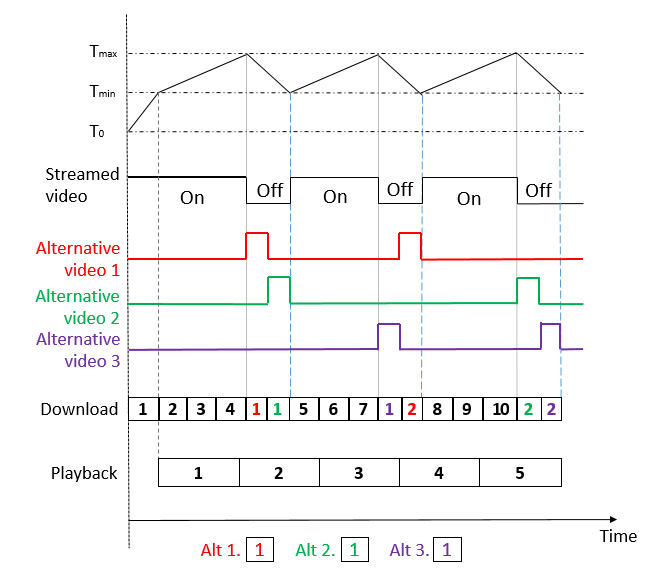
\includegraphics[scale=0.6]{prefetch.png}
	\caption{Prefetching overview}
	\label{fig:prefetch}
\end{center}
\end{figure}

\section{Server Integration}
\label{sec:serverintegration}

The SMP player is by default set to play a stream of videos located at a server supporting HTTP-streaming. For this project we use the Adobe Media Server 5 for enabling the chunked video streaming needed for our HAS functionality. Since we use a similar OSMF player that were used by Krishnamoorthi et al. \cite{hasmultipath}, the quality of prefetched chunks are adaptive to the available bandwidth \cite{hasmultipath}.

\section{Relative Placement of Geographical Points}
\label{sec:relativeplacement}

The interface accepts an arbitrary number of video streams coupled with a cardinal direction and GPS-coordinates, including latitude and longitude values. The graphical points representing these video streams should then be placed and scaled relatively to each other on the interface's geographical map, as shown in Figure \ref{fig:gpsinterface}. To accomplish this automatic placement and scaling, an algorithm was developed to calculate where the objects should be drawn to keep their relative positions between each other, so that the graphical points accurately represents the real life locations of the recordings.

\subsection{Geographical Position Algorithm}
\label{sec:geoalgorithm}

The algorithm works as follows. First, every streamer and point of interest is an object in a list. Second, the center for which all objects will be placed relative to is calculated from all the objects. This is done by checking each and every objects latitude and longitude position and take the maximum and minimum value from them as follows:

\begin{align}
\label{eq:maxandmin}
maxX &= max\{longitude_i\},  \\
minX &= min\{longitude_i\}. \nonumber
\end{align}
 
We go through every object and take the biggest and smallest longitude value. This is done similarly for \textit{maxY} and \textit{minY} but with latitude instead of longitude. When we have the maximum and minimum value of longitude and latitude the algorithm will calculate the center of the real world map's longitude-axis and latitude-axis as follows:

\begin{align}
\label{eq:center}
centerX &= \frac{maxX+minX}{2},  \\
centerY &= \frac{maxY+minY}{2}. \nonumber
\end{align}

The formula calculates the center point of all the points for the real world map where all the points will be placed relative to. Note that \textit{centerX}, \textit{maxX} and \textit{minX} is actually spherical longitude values, similar with \textit{centerY}, \textit{maxY} and \textit{minY} which is latitude values, and not flat surface x- and y-axis values. This direct translation may cause some inaccuracy. By taking half of maximum and minimum with both longitude and latitude we can get our center point as a representation of the real world map.
 
Third, when we have the center point of all points we can calculate the maximum radius that everything will scale with as follows:

\begin{align}
\label{eq:radius}
maxRadius &= max[\frac{maxX-minX}{2}, \frac{maxY-minY}{2}].
\end{align}

The calculation checks what the maximum difference is between maximum and minimum for longitude and latitude then takes that value as its \textit{maxRadius}. This is to get the correct radius for scaling and relativity.

Fourth, with the maximum radius calculated we can now place all the objects onto the geographical map. This is done by calculating each objects relative position to the center point that we calculated in equation \ref{eq:center} and translate it to x- and y-coordinates. This translation is done with the equirectangular approximation formula \cite{equi}:

\begin{align}
\label{eq:equiretangular}
deltaX &= (centerX-longitude_i)\cdot\frac{40000}{360} \\
 &\phantom{b=\,} \cdot cos((latitude_i+centerY) \cdot \frac{\pi}{360}), \nonumber\\
deltaY &= (latitude_i-centerY)\cdot\frac{40000}{360}. \nonumber
\end{align}

Here, \textit{deltaX} and \textit{deltaY} are the projected real world x- and y-distances between a coordinate and the center point with <$longitude_i$, $latitude_i$> and <\textit{centerX}, \textit{centerY}>. This method simply calculates the distance between two geographical points on the surface of a spherical area \cite{equi}. The translation is done to fit our geographical map as it represents a view on a flat plane. In the formula we approximate the earth's circumference as 40000 km. If we had used latitude and longitude as plain \textit{x} and \textit{y} values instead the positions would not have provided a good enough accuracy to the flat x-/y-plane because of the spherical nature of latitude and longitude coordinates. An alternative method of calculating the distance between two objects would have been the Haversine formula, which excels at accuracy along high distances \cite{haversine}. However, for smaller distances, as used in this project, equirectangular projection suffices.

With \textit{deltaX}, \textit{deltaY} and \textit{maxRadius} the relative distance on the display can be calculated. For calculating these relative distances, \textit{relX} and \textit{relY}, 
we first have to calculate a point's distance to the center point. For this, Pythagoras theorem is used:

\begin{align}
\label{eq:deltaZ}
deltaZ = \sqrt{deltaX^2 + deltaY^2}.
\end{align}

With \textit{deltaZ} the relative placement for the point in the x- and y-axis compared to this distance can be calculated:

\begin{align}
\label{eq:percent}
percentOfX = \frac{deltaX}{deltaZ}, \\
percentOfY = \frac{deltaY}{deltaZ}. \nonumber
\end{align}

The two values,  \textit{percentOfX} and \textit{percentOfY},  represents how many percent of \textit{deltaZ} a point is placed in the x- and y-axis. With this the only thing left to do is to calculate a scaling factor, in order to rescale the point's position according to the interface's size without losing relativity: 

\begin{align}
\label{eq:scalingFactor}
\gamma = \frac{deltaZ}{maxRadius \cdot \frac{40000}{360}}.
\end{align}

The scaling factor \textit{$\gamma$} is calculated by multiplying the \textit{maxRadius} with a constant that is used in the equirectangular formula to get the radius for x- and y-coordinates. Then we calculate how many percent of \textit{maxRadius} the distance \textit{deltaZ} is. With the scaling factor \textit{$\gamma$} a new \textit{deltaZ} can be calculated that is adapted to the interface's size:

\begin{align}
\label{eq:newZ}
relZ = \gamma \cdot Mapradius.
\end{align}

The value \textit{relZ} is the distance from the interface center point and where the point should be on the interface, and \textit{Mapradius} is the radius for the interface. To calculate how much to move the point in the x- and y-axis we only need to multiply \textit{relZ} with the percent we got from equation \ref{eq:percent}:

\begin{align}
\label{eq:newXandY}
relX = relZ \cdot percentOfX, \\
relY = relZ \cdot perecntOfY. \nonumber
\end{align}

What we basically have done is to make sure that scaling of the distances is adapted to our geographical map's boundaries. When we have the move values, \textit{relX} and \textit{relY}, the algorithm will move each object with that value from the center of the geo-map which all objects will have as its starting position. 

When executing this algorithm for geographical object placement two checks are done on all the objects to be placed. One time for equation \ref{eq:maxandmin} and one time for equations \ref{eq:equiretangular}-\ref{eq:newXandY}. Since the number of objects is \textit{n} and we go through them two times the time to execute the algorithm is $\mathcal{O}(2n)$. The constant two can be removed due to the nature of big O, making the final time complexity for the algorithm $\mathcal{O}(n)$.



\subsection{Simplification of the Algorithm}
\label{sec:limacc}

The geographical position algorithm places every object very good compared to reality in a way that relativity is kept. However, the equirectangular approximation formula that is used in equation \ref{eq:equiretangular} can be approximated. Since every object is placed with a relatively small distance between each other the algorithm can be simplified to the following: 

\begin{align*}
deltaX &= (centerX-longitude_i)\cdot\frac{40000}{360}, \\
deltaY &= (latitude_i-centerY)\cdot\frac{40000}{360}. \\
\end{align*}

The equation above is simpler and removes the \textit{cos} that was used previously because for small distances the value of \textit{cos} will be close to one. Since video streams in a real-life scenario will be very close when streaming the same point of interest the simplification does not cause any problems in relativity. The accuracy of the algorithm will be demonstrated in \textit{Chapter 4}.

\section{Technical Details}
\label{sec:technicaldetails}

To be able to accomplish switching between videos and getting a functional UI there are a lot of technical details to be explained in order to get a full understanding of how the code works. Since we used the code from Krishnamoorthi et al. \cite{qualbranch} there was first a lot to understand before we could start doing anything. The problems we had and complications we encountered will be explained \textit{Chapter 5} while the focus in this section will be on \textbf{our} code and implementations. 

\clearpage
Our progression can be divided into different sections which will be explained in a general detail:

\begin{enumerate}
\item Making a button to open the view.

\item Making a view appear, which displays a map with a point of interest and cardinal directions.

\item Making clickable geo-map objects appear on the displayed map.

\item Connecting each geo-map object to a video and be able to play it through a class called \textit{AdvertisementPluginInfo}.

\item Making the geo-map videos interactable.

%\item (Attempting to make the geo-map switching seamless.)This will be added to result/discussion instead.

\item Adjustments and improvements of the code and the implementation of a position algorithm. 
\end{enumerate}

The details of the code and implementation will not be explained line by line but a more general idea and overview will be given of what was done.

The first step was to make an interactive button which opens the graphical interface. Three different colored assets had to be created for how the button should look like, which we designed in Photoshop. The button illustrates three arrows with a dot at each end facing a general direction. This shows that a view is opened with objects similar to those. These buttons were then added to a ShockWave Component (SWC) file which stores the assets. The assets were then given an assets id and name so they could be retrieved using these as references. A class for the button was created and was added to the control bar. The button extended \textit{ButtonWidget} where it could add the assets to a "face", a kind of state, which allowed the button to switch between the different assets when changing face. 

The second step was to make a view appear that is represented as circle to better fit with how geo-map objects will be placed. For this step a widget and sprite class was created. The geo-map widget class handles the layout of the clickable layout, the creation of the geo-map view and the handling of fullscreen. The geo-map view is placed in the middle of the stage for the player and when fullscreen is initiated the graphical interface will be moved and scaled in such a way that relativity is kept. In the geo-map sprite class the position algorithm, creation of every object and cardinal direction is handled.

In the third step a new class was created called \textit{GeoMapObject} which holds all functions of the streaming video to be shown in the media player. This class have functions to add and get the position of the geo-map object, the latitude and longitude of the real life recording position, direction, setting the video stream URL to be connected with the object etc. The geo-map object which is created in the geo-map sprite class is added to a list. This list will handle all the geo-map objects on the view and is used for when clicking on an object. Together with a function in the geo-map object class it helps to show which object is clicked on and make sure that no more than one object is highlighted at the same time.

Continuing to the fourth step, the technicalities became a bit more complicated and this is the part when the servers came into play and getting the videos to show up on the media player. More details about the server will be explained in \textit{Section} \ref{sec:server}. For this step each video in the geo-map objects needed to be played with a class called \textit{AdvertisementPluginInfo}, which is a class created for the purpose of playing advertisement videos in the beginning, middle or end of a video. In this stage, modifications were done to the functionality of the \textit{AdvertisementPluginInfo} class from instead of playing the video acting as an advertisement halfway through the main video, to play the video acting as an advertisement at the start of the main video stream. This allows for the switch to happen directly when the geo-map object is clicked on. However, to get this to work the class also needed to first stop the main video and signal that another video is playing. For this the main media player from the Strobe Media Playback needed to be fetched and sent in to the \textit{AdvertisementPluginInfo} class as a reference. This was solved by creating the geo-map button in the SMP class and then sending the reference which was forwarded to the geo-map objects. This way the media container and media player that the SMP intitially used could be stopped and removed. When this was done the \textit{AdvertisementPluginInfo} class could change between the different videos, as if they were multiple advertisements, which meant that only playing the advertisement videos was possible but not being able to interact with them. 

Step five, which was about getting the interaction for the videos to work, was the most difficult task of them all. Since the videos were played as an advertisement some things needed to be changed, because these advertisement videos was set to not be interactable through the user interface. The main thing here is that the media player still recognizes the non-advertisement video as the main media from the Strobe Media Playback while the geo-map interface's videos was only some advertisements on top of it. What was done to fix this was to rewire all of the graphical user interface in a way that you would be able to control the advertisements with it. In other words instead of playing, pausing and interacting with the user interface for the main video, a check is done for the controls. What this check does is that it checks if an "advertisement" is being played and if it is, then the controls will be changed to affect the advertisement instead.

In the last step adjustments and improvements was done to the code and also the implementation of the position algorithm. Here the code was adjusted and improved to make sure that the implementations which were done would not crash anything else. Here, the \textit{PointOfInterest} class was implemented to better fit the relative position algorithm. Since the algorithm uses a list of all geo-map objects there was need for \textit{PointOfInterest} to be an object that uses similar functions to the ones in the geo-map object class. 

\section{Server and Video Application}
\label{sec:server}

As previously mentioned in the report the server used is the Adobe Media Server 5 (AMS 5), which is primary used for downloading videos from cache as similar to the works described in \textit{Chapter 2}. AMS 5 is a server used for HTTP-streaming which is needed in order to use HAS. The AMS 5 uses something called an Apache server, specifically Apache 2.4, which enables a video to be called with HTTP. To stream videos with the AMS 5 there can be a need to allow the the flash player to stream a HTTP-video through the local media player\footnote{Global\:Security\:Settings\:panel: https://www.macromedia.com/support/documentation/en/\\flashplayer/help/settings$\_$manager04.html}, otherwise security errors may occur. The reason for this security error being that a call is made in the code to a plug-in which allows for sending and requesting a URL to be played.

Except for using the AMS 5 to play a video through HTTP the video also needs to be in formats of F4V or FLV which are two different video file formats commonly used for delivering videos over internet using Adobe Flash Player. Every recorded video for this thesis has been converted to FLV with FFmpeg\footnote{FFmpeg: https://ffmpeg.org/} which is a free open source software project including libraries and utilities for converting multimedia data.

